\documentclass[a4paper]{article}

\def\nterm {Spring}
\def\nyear {2020}
\def\nlecturer {Dan Perelstein}
\def\ncourse {Sound Systems Design and Engineering}

\RequirePackage{etex}
\makeatletter
\ifx \nauthor\undefined
  \def\nauthor{Daniel Moore}
\else
\fi

\author{Based on lectures by \nlecturer \\\small Notes taken by \nauthor}
\date{\nterm\ \nyear}

\usepackage{alltt}
\usepackage{amsfonts}
\usepackage{amsmath}
\usepackage{amssymb}
\usepackage{amsthm}
\usepackage{booktabs}
\usepackage[makeroom]{cancel}
\usepackage{caption}
\usepackage{enumitem}
\usepackage{fancyhdr}
\usepackage{graphicx}
\usepackage{mathdots}
\usepackage{mathtools}
\usepackage{microtype}
\usepackage{multirow}
\usepackage{pdflscape}
\usepackage{pgfplots}
\usepackage{siunitx}
\usepackage{textcomp}
\usepackage{slashed}
\usepackage{tabularx}
\usepackage{tikz}
\usepackage{tikz-3dplot}
\usepackage{tkz-euclide}
\usepackage{titlesec}
\usepackage[normalem]{ulem}
\usepackage[all]{xy}
\usepackage{imakeidx}

\makeindex[intoc, title=Index]
\indexsetup{othercode={\lhead{\emph{Index}}}}
%\setcounter{secnumdepth}{4}

\titleformat{\paragraph}
{\normalfont\normalsize\bfseries}{\theparagraph}{1em}{}
\titlespacing*{\paragraph}
{0pt}{3.25ex plus 1ex minus .2ex}{1.5ex plus .2ex}

\ifx \nextra \undefined
  \usepackage[pdftex,
    hidelinks,
    pdfauthor={Daniel Moore},
    pdfsubject={\ncourse},
    pdftitle={\ncourse},
  pdfkeywords={\nterm\ \nyear\ \ncourse}]{hyperref}
  \title{\ncourse}
\else
  \usepackage[pdftex,
    hidelinks,
    pdfauthor={Daniel Moore},
    pdfsubject={\ncourse\ (\nextra)},
    pdftitle={\ncourse\ (\nextra)},
  pdfkeywords={\nterm\ \nyear\ \ncourse\ \nextra}]{hyperref}

  \title{\ncourse \\ {\Large \nextra}}
  \renewcommand\printindex{}
\fi

\pgfplotsset{compat=1.12}

\pagestyle{fancyplain}
\ifx \ncoursehead \undefined
\def\ncoursehead{\ncourse}
\fi

\lhead{\emph{\nouppercase{\leftmark}}}
\ifx \nextra \undefined
  \rhead{
    \ifnum\thepage=1
    \else
      \ncoursehead
    \fi}
\else
  \rhead{
    \ifnum\thepage=1
    \else
      \ncoursehead \ (\nextra)
    \fi}
\fi
\usetikzlibrary{arrows.meta}
\usetikzlibrary{decorations.markings}
\usetikzlibrary{decorations.pathmorphing}
\usetikzlibrary{positioning}
\usetikzlibrary{fadings}
\usetikzlibrary{intersections}
\usetikzlibrary{cd}

\newcommand*{\Cdot}{{\raisebox{-0.25ex}{\scalebox{1.5}{$\cdot$}}}}
\newcommand {\pd}[2][ ]{
  \ifx #1 { }
    \frac{\partial}{\partial #2}
  \else
    \frac{\partial^{#1}}{\partial #2^{#1}}
  \fi
}
\newcommand{\pder}[2]{
    \frac{\partial #1}{\partial #2}
}
\newcommand{\dd}[1]{
	\frac{\d}{\d #1}
}
\newcommand{\der}[2]{
	\frac{\d #1}{\d #2}
}
\newcommand{\mbeq}{\overset{!}{=}}
\newcommand{\vhat}[1]{\vec{\hat{#1}}}
\newcommand{\x}{\vhat{x}}
\newcommand{\y}{\vhat{y}}
\newcommand{\z}{\vhat{z}}
\newcommand{\del}{\vec{\nabla}}
\ifx \nhtml \undefined
\else
  \renewcommand\printindex{}
  \DisableLigatures[f]{family = *}
  \let\Contentsline\contentsline
  \renewcommand\contentsline[3]{\Contentsline{#1}{#2}{}}
  \renewcommand{\@dotsep}{10000}
  \newlength\currentparindent
  \setlength\currentparindent\parindent

  \newcommand\@minipagerestore{\setlength{\parindent}{\currentparindent}}
  \usepackage[active,tightpage,pdftex]{preview}
  \renewcommand{\PreviewBorder}{0.1cm}

  \newenvironment{stretchpage}%
  {\begin{preview}\begin{minipage}{\hsize}}%
    {\end{minipage}\end{preview}}
  \AtBeginDocument{\begin{stretchpage}}
  \AtEndDocument{\end{stretchpage}}

  \newcommand{\@@newpage}{\end{stretchpage}\begin{stretchpage}}

  \let\@real@section\section
  \renewcommand{\section}{\@@newpage\@real@section}
  \let\@real@subsection\subsection
  \renewcommand{\subsection}{\@ifstar{\@real@subsection*}{\@@newpage\@real@subsection}}
\fi
\ifx \ntrim \undefined
\else
  \usepackage{geometry}
  \geometry{
    papersize={379pt, 699pt},
    textwidth=345pt,
    textheight=596pt,
    left=17pt,
    top=54pt,
    right=17pt
  }
\fi

\ifx \nisofficial \undefined
\let\@real@maketitle\maketitle
\renewcommand{\maketitle}{\@real@maketitle\begin{center}\begin{minipage}[c]{0.9\textwidth}\centering\footnotesize These notes are not endorsed by the lecturers, and I have modified them (often significantly) after lectures. They are nowhere near accurate representations of what was actually lectured, and in particular, all errors are almost surely mine.\end{minipage}\end{center}}
\else
\fi

% Theorems
\theoremstyle{definition}
\newtheorem*{aim}{Aim}
\newtheorem*{axiom}{Axiom}
\newtheorem*{claim}{Claim}
\newtheorem*{cor}{Corollary}
\newtheorem*{conjecture}{Conjecture}
\newtheorem*{defi}{Definition}
\newtheorem*{eg}{Example}
\newtheorem*{ex}{Exercise}
\newtheorem*{fact}{Fact}
\newtheorem*{law}{Law}
\newtheorem*{lemma}{Lemma}
\newtheorem*{notation}{Notation}
\newtheorem*{prop}{Proposition}
\newtheorem*{question}{Question}
\newtheorem*{problem}{Problem}
\newtheorem*{rrule}{Rule}
\newtheorem*{thm}{Theorem}
\newtheorem*{assumption}{Assumption}

\newtheorem*{remark}{Remark}
\newtheorem*{warning}{Warning}
\newtheorem*{exercise}{Exercise}

\newtheorem{nthm}{Theorem}[section]
\newtheorem{nlemma}[nthm]{Lemma}
\newtheorem{nprop}[nthm]{Proposition}
\newtheorem{ncor}[nthm]{Corollary}


\renewcommand{\labelitemi}{--}
\renewcommand{\labelitemii}{$\circ$}
\renewcommand{\labelenumi}{(\roman{*})}

\let\stdsection\section
\renewcommand\section{\newpage\stdsection}

% Strike through
\def\st{\bgroup \ULdepth=-.55ex \ULset}


%%%%%%%%%%%%%%%%%%%%%%%%%
%%%%% Maths Symbols %%%%%
%%%%%%%%%%%%%%%%%%%%%%%%%

% Matrix groups
\newcommand{\GL}{\mathrm{GL}}
\newcommand{\Or}{\mathrm{O}}
\newcommand{\PGL}{\mathrm{PGL}}
\newcommand{\PSL}{\mathrm{PSL}}
\newcommand{\PSO}{\mathrm{PSO}}
\newcommand{\PSU}{\mathrm{PSU}}
\newcommand{\SL}{\mathrm{SL}}
\newcommand{\SO}{\mathrm{SO}}
\newcommand{\Spin}{\mathrm{Spin}}
\newcommand{\Sp}{\mathrm{Sp}}
\newcommand{\SU}{\mathrm{SU}}
\newcommand{\U}{\mathrm{U}}
\newcommand{\Mat}{\mathrm{Mat}}

% Matrix algebras
\newcommand{\gl}{\mathfrak{gl}}
\newcommand{\ort}{\mathfrak{o}}
\newcommand{\so}{\mathfrak{so}}
\newcommand{\su}{\mathfrak{su}}
\newcommand{\uu}{\mathfrak{u}}
\renewcommand{\sl}{\mathfrak{sl}}

% Special sets
\newcommand{\C}{\mathbb{C}}
\newcommand{\CP}{\mathbb{CP}}
\newcommand{\GG}{\mathbb{G}}
\newcommand{\N}{\mathbb{N}}
\newcommand{\Q}{\mathbb{Q}}
\newcommand{\R}{\mathbb{R}}
\newcommand{\RP}{\mathbb{RP}}
\newcommand{\T}{\mathbb{T}}
\newcommand{\Z}{\mathbb{Z}}
\renewcommand{\H}{\mathbb{H}}

% Brackets
\newcommand{\abs}[1]{\left\lvert #1\right\rvert}
\newcommand{\bket}[1]{\left\lvert #1\right\rangle}
\newcommand{\brak}[1]{\left\langle #1 \right\rvert}
\newcommand{\braket}[2]{\left\langle #1\middle\vert #2 \right\rangle}
\newcommand{\bra}{\langle}
\newcommand{\ket}{\rangle}
\newcommand{\norm}[1]{\left\lVert #1\right\rVert}
\newcommand{\normalorder}[1]{\mathop{:}\nolimits\!#1\!\mathop{:}\nolimits}
\newcommand{\tv}[1]{|#1|}
\renewcommand{\vec}[1]{\boldsymbol{\mathbf{#1}}}

% not-math
\newcommand{\bolds}[1]{{\bfseries #1}}
\newcommand{\cat}[1]{\mathsf{#1}}
\newcommand{\ph}{\,\cdot\,}
\newcommand{\term}[1]{\emph{#1}\index{#1}}
\newcommand{\phantomeq}{\hphantom{{}={}}}
% Probability
\DeclareMathOperator{\Bernoulli}{Bernoulli}
\DeclareMathOperator{\betaD}{beta}
\DeclareMathOperator{\bias}{bias}
\DeclareMathOperator{\binomial}{binomial}
\DeclareMathOperator{\corr}{corr}
\DeclareMathOperator{\cov}{cov}
\DeclareMathOperator{\gammaD}{gamma}
\DeclareMathOperator{\mse}{mse}
\DeclareMathOperator{\multinomial}{multinomial}
\DeclareMathOperator{\Poisson}{Poisson}
\DeclareMathOperator{\var}{var}
\newcommand{\E}{\mathbb{E}}
\newcommand{\Prob}{\mathbb{P}}

% Algebra
\DeclareMathOperator{\adj}{adj}
\DeclareMathOperator{\Ann}{Ann}
\DeclareMathOperator{\Aut}{Aut}
\DeclareMathOperator{\Char}{char}
\DeclareMathOperator{\disc}{disc}
\DeclareMathOperator{\dom}{dom}
\DeclareMathOperator{\fix}{fix}
\DeclareMathOperator{\Hom}{Hom}
\DeclareMathOperator{\id}{id}
\DeclareMathOperator{\image}{image}
\DeclareMathOperator{\im}{im}
\DeclareMathOperator{\re}{re}
\DeclareMathOperator{\tr}{tr}
\DeclareMathOperator{\Tr}{Tr}
\newcommand{\Bilin}{\mathrm{Bilin}}
\newcommand{\Frob}{\mathrm{Frob}}

% Others
\newcommand\ad{\mathrm{ad}}
\newcommand\Art{\mathrm{Art}}
\newcommand{\B}{\mathcal{B}}
\newcommand{\cU}{\mathcal{U}}
\newcommand{\Der}{\mathrm{Der}}
\newcommand{\D}{\mathrm{D}}
\newcommand{\dR}{\mathrm{dR}}
\newcommand{\exterior}{\mathchoice{{\textstyle\bigwedge}}{{\bigwedge}}{{\textstyle\wedge}}{{\scriptstyle\wedge}}}
\newcommand{\F}{\mathbb{F}}
\newcommand{\G}{\mathcal{G}}
\newcommand{\Gr}{\mathrm{Gr}}
\newcommand{\haut}{\mathrm{ht}}
\newcommand{\Hol}{\mathrm{Hol}}
\newcommand{\hol}{\mathfrak{hol}}
\newcommand{\I}{\mathbb{I}}
\newcommand{\Id}{\mathrm{Id}}
\newcommand{\Lp}{\mathcal{L}}
\newcommand{\lie}[1]{\mathfrak{#1}}
\newcommand{\op}{\mathrm{op}}
\newcommand{\Oc}{\mathcal{O}}
\newcommand{\pr}{\mathrm{pr}}
\newcommand{\Ps}{\mathcal{P}}
\newcommand{\pt}{\mathrm{pt}}
\newcommand{\qeq}{\mathrel{``{=}"}}
\newcommand{\Rs}{\mathcal{R}}
\newcommand{\Vect}{\mathrm{Vect}}
\newcommand{\wsto}{\stackrel{\mathrm{w}^*}{\to}}
\newcommand{\wt}{\mathrm{wt}}
\newcommand{\wto}{\stackrel{\mathrm{w}}{\to}}
\renewcommand{\d}{\mathrm{d}}
\renewcommand{\P}{\mathbb{P}}
%\renewcommand{\F}{\mathcal{F}}


\let\Im\relax
\let\Re\relax

\DeclareMathOperator{\area}{area}
\DeclareMathOperator{\card}{card}
\DeclareMathOperator{\ccl}{ccl}
\DeclareMathOperator{\ch}{ch}
\DeclareMathOperator{\cl}{cl}
\DeclareMathOperator{\cls}{\overline{\mathrm{span}}}
\DeclareMathOperator{\coker}{coker}
\DeclareMathOperator{\conv}{conv}
\DeclareMathOperator{\cosec}{cosec}
\DeclareMathOperator{\cosech}{cosech}
\DeclareMathOperator{\covol}{covol}
\DeclareMathOperator{\diag}{diag}
\DeclareMathOperator{\diam}{diam}
\DeclareMathOperator{\Diff}{Diff}
\DeclareMathOperator{\End}{End}
\DeclareMathOperator{\energy}{energy}
\DeclareMathOperator{\erfc}{erfc}
\DeclareMathOperator{\erf}{erf}
\DeclareMathOperator*{\esssup}{ess\,sup}
\DeclareMathOperator{\ev}{ev}
\DeclareMathOperator{\Ext}{Ext}
\DeclareMathOperator{\fst}{fst}
\DeclareMathOperator{\Fit}{Fit}
\DeclareMathOperator{\Frac}{Frac}
\DeclareMathOperator{\Gal}{Gal}
\DeclareMathOperator{\gr}{gr}
\DeclareMathOperator{\hcf}{hcf}
\DeclareMathOperator{\Im}{Im}
\DeclareMathOperator{\Ind}{Ind}
\DeclareMathOperator{\Int}{Int}
\DeclareMathOperator{\Isom}{Isom}
\DeclareMathOperator{\lcm}{lcm}
\DeclareMathOperator{\length}{length}
\DeclareMathOperator{\Lie}{Lie}
\DeclareMathOperator{\like}{like}
\DeclareMathOperator{\Lk}{Lk}
\DeclareMathOperator{\Maps}{Maps}
\DeclareMathOperator{\orb}{orb}
\DeclareMathOperator{\ord}{ord}
\DeclareMathOperator{\otp}{otp}
\DeclareMathOperator{\poly}{poly}
\DeclareMathOperator{\rank}{rank}
\DeclareMathOperator{\rel}{rel}
\DeclareMathOperator{\Rad}{Rad}
\DeclareMathOperator{\Re}{Re}
\DeclareMathOperator*{\res}{res}
\DeclareMathOperator{\Res}{Res}
\DeclareMathOperator{\Ric}{Ric}
\DeclareMathOperator{\rk}{rk}
\DeclareMathOperator{\Rees}{Rees}
\DeclareMathOperator{\Root}{Root}
\DeclareMathOperator{\sech}{sech}
\DeclareMathOperator{\sgn}{sgn}
\DeclareMathOperator{\snd}{snd}
\DeclareMathOperator{\Spec}{Spec}
\DeclareMathOperator{\spn}{span}
\DeclareMathOperator{\stab}{stab}
\DeclareMathOperator{\St}{St}
\DeclareMathOperator{\supp}{supp}
\DeclareMathOperator{\Syl}{Syl}
\DeclareMathOperator{\Sym}{Sym}
\DeclareMathOperator{\vol}{vol}

\pgfarrowsdeclarecombine{twolatex'}{twolatex'}{latex'}{latex'}{latex'}{latex'}
\tikzset{->/.style = {decoration={markings,
                                  mark=at position 1 with {\arrow[scale=2]{latex'}}},
                      postaction={decorate}}}
\tikzset{<-/.style = {decoration={markings,
                                  mark=at position 0 with {\arrowreversed[scale=2]{latex'}}},
                      postaction={decorate}}}
\tikzset{<->/.style = {decoration={markings,
                                   mark=at position 0 with {\arrowreversed[scale=2]{latex'}},
                                   mark=at position 1 with {\arrow[scale=2]{latex'}}},
                       postaction={decorate}}}
\tikzset{->-/.style = {decoration={markings,
                                   mark=at position #1 with {\arrow[scale=2]{latex'}}},
                       postaction={decorate}}}
\tikzset{-<-/.style = {decoration={markings,
                                   mark=at position #1 with {\arrowreversed[scale=2]{latex'}}},
                       postaction={decorate}}}
\tikzset{->>/.style = {decoration={markings,
                                  mark=at position 1 with {\arrow[scale=2]{latex'}}},
                      postaction={decorate}}}
\tikzset{<<-/.style = {decoration={markings,
                                  mark=at position 0 with {\arrowreversed[scale=2]{twolatex'}}},
                      postaction={decorate}}}
\tikzset{<<->>/.style = {decoration={markings,
                                   mark=at position 0 with {\arrowreversed[scale=2]{twolatex'}},
                                   mark=at position 1 with {\arrow[scale=2]{twolatex'}}},
                       postaction={decorate}}}
\tikzset{->>-/.style = {decoration={markings,
                                   mark=at position #1 with {\arrow[scale=2]{twolatex'}}},
                       postaction={decorate}}}
\tikzset{-<<-/.style = {decoration={markings,
                                   mark=at position #1 with {\arrowreversed[scale=2]{twolatex'}}},
                       postaction={decorate}}}

\tikzset{circ/.style = {fill, circle, inner sep = 0, minimum size = 3}}
\tikzset{scirc/.style = {fill, circle, inner sep = 0, minimum size = 1.5}}
\tikzset{mstate/.style={circle, draw, blue, text=black, minimum width=0.7cm}}

\tikzset{eqpic/.style={baseline={([yshift=-.5ex]current bounding box.center)}}}
\tikzset{commutative diagrams/.cd,cdmap/.style={/tikz/column 1/.append style={anchor=base east},/tikz/column 2/.append style={anchor=base west},row sep=tiny}}

\definecolor{mblue}{rgb}{0.2, 0.3, 0.8}
\definecolor{morange}{rgb}{1, 0.5, 0}
\definecolor{mgreen}{rgb}{0.1, 0.4, 0.2}
\definecolor{mred}{rgb}{0.5, 0, 0}

\def\drawcirculararc(#1,#2)(#3,#4)(#5,#6){%
    \pgfmathsetmacro\cA{(#1*#1+#2*#2-#3*#3-#4*#4)/2}%
    \pgfmathsetmacro\cB{(#1*#1+#2*#2-#5*#5-#6*#6)/2}%
    \pgfmathsetmacro\cy{(\cB*(#1-#3)-\cA*(#1-#5))/%
                        ((#2-#6)*(#1-#3)-(#2-#4)*(#1-#5))}%
    \pgfmathsetmacro\cx{(\cA-\cy*(#2-#4))/(#1-#3)}%
    \pgfmathsetmacro\cr{sqrt((#1-\cx)*(#1-\cx)+(#2-\cy)*(#2-\cy))}%
    \pgfmathsetmacro\cA{atan2(#2-\cy,#1-\cx)}%
    \pgfmathsetmacro\cB{atan2(#6-\cy,#5-\cx)}%
    \pgfmathparse{\cB<\cA}%
    \ifnum\pgfmathresult=1
        \pgfmathsetmacro\cB{\cB+360}%
    \fi
    \draw (#1,#2) arc (\cA:\cB:\cr);%
}
\newcommand\getCoord[3]{\newdimen{#1}\newdimen{#2}\pgfextractx{#1}{\pgfpointanchor{#3}{center}}\pgfextracty{#2}{\pgfpointanchor{#3}{center}}}

\newcommand\qedshift{\vspace{-17pt}}
\newcommand\fakeqed{\pushQED{\qed}\qedhere}

\def\Xint#1{\mathchoice
   {\XXint\displaystyle\textstyle{#1}}%
   {\XXint\textstyle\scriptstyle{#1}}%
   {\XXint\scriptstyle\scriptscriptstyle{#1}}%
   {\XXint\scriptscriptstyle\scriptscriptstyle{#1}}%
   \!\int}
\def\XXint#1#2#3{{\setbox0=\hbox{$#1{#2#3}{\int}$}
     \vcenter{\hbox{$#2#3$}}\kern-.5\wd0}}
\def\ddashint{\Xint=}
\def\dashint{\Xint-}

\newcommand\separator{{\centering\rule{2cm}{0.2pt}\vspace{2pt}\par}}

\newenvironment{own}{\color{gray!70!black}}{}

\newcommand\makecenter[1]{\raisebox{-0.5\height}{#1}}

\mathchardef\mdash="2D

\newenvironment{significant}{\begin{center}\begin{minipage}{0.9\textwidth}\centering\em}{\end{minipage}\end{center}}
\DeclareRobustCommand{\rvdots}{%
  \vbox{
    \baselineskip4\p@\lineskiplimit\z@
    \kern-\p@
    \hbox{.}\hbox{.}\hbox{.}
  }}
\DeclareRobustCommand\tph[3]{{\texorpdfstring{#1}{#2}}}
\makeatother


\begin{document}
\maketitle

\tableofcontents
\clearpage

\part{Loudspeakers}

\section{System Design Building Blocks}
\subsection{Decibel Math}
The decibel (dB) involves the use of a logarithm to allow large differences and
numbers to be written as conveniently small numbers. A decibel is a ratio
between two pressure levels (ie. the measure of deviation of air at a certain
point due to sound). These get big so quickly that logarithms quickly become
necessary.

There are two definitions for decibels:
\begin{align*}
	\mathrm{dB} &= 10\log_{10}\left(\frac{A}{B}\right)\\
	\mathrm{dB} &= 20\log_{10}\left(\frac{A}{B}\right)
\end{align*}
The first definition is in reference to power, the second in reference to
voltage. In this class, we'll only work with the second one, as that's the one
that is generally useful for sound. The first one is useful when talking about
power amplifiers. For the future, we'll write $\log$ instead of $\log_{10}$ for
the sake of simplicity.

$A$ is the pressure value we want to measure, and $B$ is the reference value.
The reference value we use ($B$) is the quietest sound that it's possible to
hear.

\subsubsection{Logarithms (and their Applications)}
A base-10 logarithm like we'll be using answers the question ``what exponent
does 10 need to be raised to to equal our value?''
For example, $10^1 = 10$, so
\[
	\log(10) = 1
\]
This asks the question ``what exponent does 10 need to be raised to to equal
10,'' for which the answer is 1.
Another example, $10^0 = 1$, so
\[
	\log(1) = 0
\]
This asks the question ``what expoent does 10 need to be raised to to equal
1,'' for which the answer is zero.

Logarithms convert multiplication into simple addition and division into simple
subtraction. Written out, what this means is that we can write $\log(AB)$
instead as
\[
	\log(AB) = \log(A) + \log(B)
\]
Similarly, we can also write $\log(A/B)$ as
\[
	\log\left(\frac{A}{B}\right) = \log(A) - \log(B)
\]

There's another important thing to note about logarithms. If we measure the
sound pressure level (SPL) at some point to be $x$ dB, that means that we know
\[
	x = 20\log\left(\frac{A}{B}\right)
\]
How do the number of decibels change for a sound twice as strong?
\begin{align*}
	20\log\left(2\frac{A}{B}\right)
	&= 20\log(2) + 20\log\left(\frac{A}{B}\right)\\
	&= 20\log(2) + x\\
	&= 20(.03) + x\\
	&= 6 \mathrm{dB} + x \mathrm{dB}
\end{align*}
What this means is that any time we double the pressure of the sound, we're
adding $6$ dB.\\
Let's see what happens if we do this but we half it instead:
\begin{align*}
	20\log\left(\frac{1}{2}\frac{A}{B}\right) &= 
	20\log\left(\frac{A}{2B}\right)\\
	&= 20\log\left(\frac{A}{B}\right) - 20\log(2)\\
	&= x \mathrm{dB} - 6 \mathrm{dB}
\end{align*}
So, halving the pressure level means we subtract $6$ dB.\\
One more example: what happens if we have an SPL ten times as large?
\begin{align*}
	20\log\left(10\frac{A}{B}\right) &=
	20\log(10) + 20\log\left(\frac{A}{B}\right)\\
	&= 20(1) + x\\
	&= 20 \mathrm{dB} + x \mathrm{dB}
\end{align*}
This means that to get a sound with ten times the pressure, we have to add
exactly 20 dB.

\subsection{Inverse Square Law}
As an introduction, the surface area of a sphere is
\[
	\text{Surface Area} = 4\pi r^2
\]
where $r$ is the radius of a sphere. Note that if we double the radius, there
will be 4 times as much surface area.

The inverse square law isn't just a sound thing---it's common between sound,
gravitational pull, electric field strength, radiation, etc. If we have a point
source that obeys the inverse square law (imagine, for example, a speaker in
the air broadcasting sound equally in all directions), the intensity of a sound
is inversly proportional to the distance from the source (as distance
increases, intensity decreases, and visa-versa). Specifically, they're
inversely proportional with a square relationship (hence the name). For
example, if we move away from the source a distance of 2m, the intensity drops
to 1/4 of what it was. This is because the sound is being projected in a
sphere, and as we get farther away, the surface area is increasing, but the
total sound pressure isn't increasing, so the sound has to spread out more to
cover the area.

As an example. If a speaker 1 ft away from you has volume $x$. At 2 ft, it
would have volume of $\frac{1}{4}x$. At 3 ft, $\frac{1}{9}x$. At 4 ft,
$\frac{1}{16}x$. And so on. We get these numbers by squaring the distance and
putting it on the bottom.

An important conclusion from this: if you're using surround sound (ie. sound
from behind the audience), you'll get more even coverage if you put the
speakers farther behind the audience. If the speakers are, for example, 1 ft
behind the back of the audience, the volume even 6 feet away (one or 2 rows up)
will be already $\frac{1}{36}$ the intensity since it's 6 times as far.
On the other hand, if we put the
speakers 12 ft away from the last audience member, the volume 6 feet away (one
or 2 rows up) is only 1.5 times as far away, so it's only $\frac{4}{9}$ as
quiet (if I'm doing my math right). This still isn't the best, but it's a lot
better. We can also use vertical height to increase the distance from the
audience without having to go as far back.

\subsection{Reference Signals}
\subsubsection{Sine Waves}
Sine waves are patterns of air pressure where the pressure in some direction
can be modelled using a sine curve (very generally, this means that areas of
high pressure happen at regular, predictable intervals at regular, predictable
maximum intensities, and areas of low pressure similarly happen at regular,
predictable intervals and with regular, predictable minimum intensities).

\subsubsection{Fourier}
Fourier found in the 1820s that any signal, no matter how
complicated, can be written as the sume of sine waves at different amplitudes
and at different phase relationships. Through Fourier analysis, we can convert
from looking at a signal as a function of time, to looking at a signal as a
function of frequency. Theoretically, we could totally replicate anything we
hear or record with a sum of sine waves, but that would take literally tens of
thousands of sine waves every moment, so it's hard.

\subsubsection{Noise}
There's two types of reference noise we use: white noise and pink noise. White
noise has more audible high end than pink noise, and pink noise has more
audible low-end. White noise has equal amplitude at every frquency. Pink noise
takes white noise and applies a ``pinking'' filter, which takes away 3 dB per
octave. There are more frequencies at a given octave at high frequencies, so in
white noise, the high frequencies have much, much more energy, making them
overpower the lower octaves. The goal with pink noise is to give us something
that sounds like it's evenly distributed betwen notes.
Here's the difference between white and pink noise (respectively) on a frequency
spectrum:\\
\begin{center}
	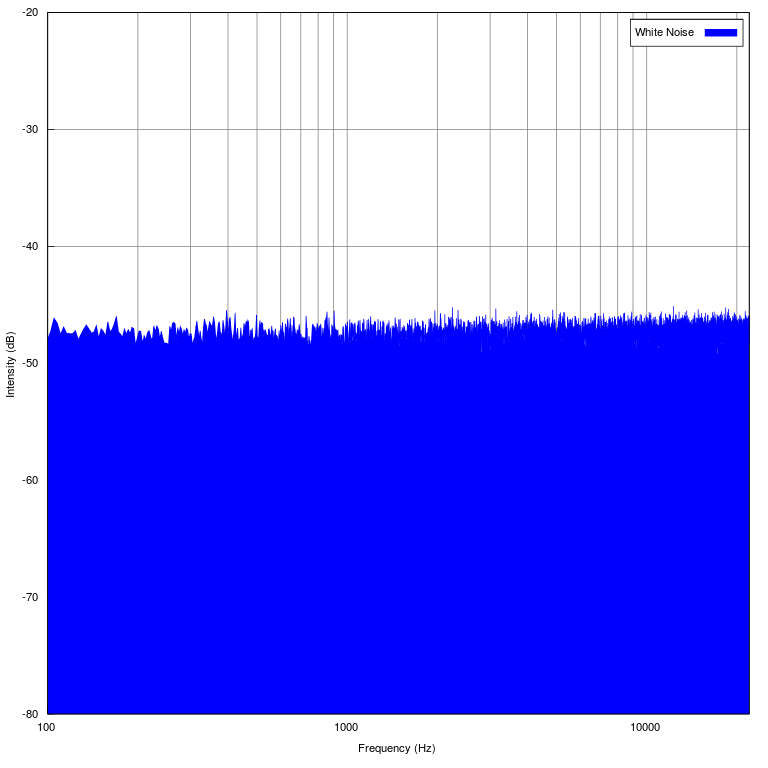
\includegraphics[width=0.45\textwidth]{WhiteNoise.png}
	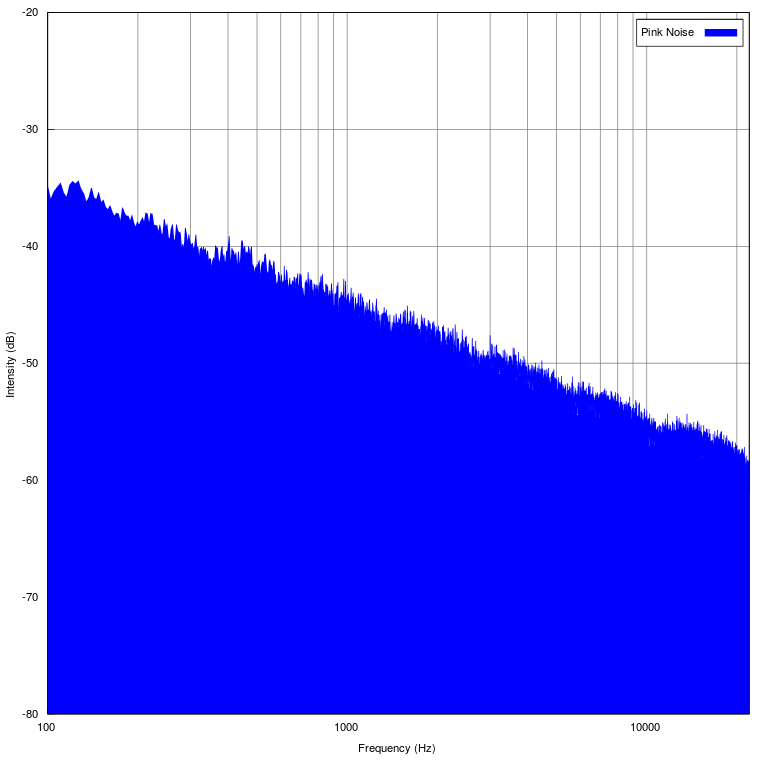
\includegraphics[width=0.45\textwidth]{PinkNoise.png}
\end{center}

\section{Loudspeakers}
\subsection{An Introduction to Loudspeakers}
Speakers are transducers: electronic components that convert one type of signal
to another. Specifically, speakers convert signals from electrical energy to
mechanical/acoustic energy.

Ideally, we want to be able to produce every sound that humans can hear (20 Hz
to 20 kHz) so we can recreate the sounds we're trying to represent as
accurately as possible. This is usually not really possible

\subsection{The -6 dB Point}
Remember that -6 dB represents halving the sound pressure level (SPL) of a
signal. The width that the manufacturers give for a loudspeaker is generally
going to e the point at which the volume is 6 dB lower than it is at the same
distance on-axis. These levels are measured at 1 kHz, since the
high-frequencies attenuate at different rates than low frequencies when you're
going off-axis. If we want even coverage, we want to line up the 6 dB point of
one loudspeaker with the 6 dB point of the other. If we overlap too much, we'll
get areas with more than 0 dB, and if we separate them too much, we'll get
areas with less than 6 dB.

\section{Vertical Coverage and Tilt}
We generally want to range of audience experiences to be within 6 dB, as much
as possible. Putting speakers vertically exactly on-axis can make that really
difficult if we don't have a very long spacec, because the front audience
member very close to the speaker and like 6 audience members back might have a
-12 dB difference. There's two things we can do to fix that: first, we can move
vertically instead of horizontally. Then, the distance from the nearest
audience member and the distance to the farthest audience member is closer to
being the same. Similarly, if we have the space, we can try to move it
horizontally farther away. That way, the ratio of distance between the closest
and farthest audience member is only 1:2 instead of 1:4 or something.

We should try to aim or speakers such that they are pointed at the farthest
audience member in the vertical plane. For a raked audience, this usually menas
pointing at the top/back row. We want to try to create a situation where gain
differences due to axial position and distance compensate for each other.

\subsection{Fill Systems}
\subsubsection{Downfill}

\subsubsection{Front Fill}
If the stage is tall, or downfill speakers would make the imaging very strange
(that is, would make a person's voice sound like it's coming from unreasonably
high rather than from themselves), we can instead use a front fill speaker or
system. Front fill speakers are placed directly in front of the audience, with
their axis pointed at the highest relavent audience memeber out of coverage
from the main speaker. In a standard theatre, front fill speakers can only
cover about the first three rows. We need to take the same frequency response
differences into consideration as with downfill speakers.

\subsubsection{Delay}
What if we're not out of axial coverage, but out of distance coverage? We can
extend the coverage of the main loudspeaker by adding another loudspeaker where
we lose coverage (at the 6 dB point). We want in this case to aim not
necessarily for the objectively highest audience member, but the highest
audience member that we're aiming for with that speaker. This additional
distance fill speaker is called a delay speaker (or a delay system, if we have
multiple). We call it a delay speaker becase we'll have to delay the signal
going to it to account for how slowly sound moves through air.\\
There are some holes in frequency response, so we will have to include both
high %CHECK
and low frequencies.

\subsubsection{A Rule of Thumb for Number of Speakers}

We can figure out roughly how many speakers we need with Bob McCarthy's formula
\[
	\frac{\text{Distance to the farthest person}}{\text{Distance to the
	closest person}} - 1
\]
This also tracks if we think in terms of decibels: for example, if this formula
gives us $1$ because of a $2:1$ ratio, that means there's a $-6 \mathrm{dB}$
difference from the closest to the nearest, so we only need one speaker.

\subsubsection{Output Delay}

Sound is unique from stuff like light because it's really slow. Light, for
example, moves at about $3,000,000$ m/s, whereas sound only travels at $340.29$
m/s, or roughly $1,000$ ft/s, or $1$ ft/ms.
In the time that it would take a beam of light to go around the Earth, a
sound would only go about $150$ feet.\\
Especially when we're talking about delay speakers or systems, we need to pay
attention to this: we need to add delay equal to the time it takes for the
sound from the main speaker to reach the delay speaker.

\section[Horizontal Coverage]{Comb-Filtering: Coverage in the Horizontal Plane}

\subsection{Phasing/Comb-Filtering}

When you hear the same sound from 2 different loudspeakers, or you pick up the
sound from two different microphones, it sounds bad in unpredictable ways. As
much as possible, we want our sounds to be heard from only one loudspeaker, and
we want our sounds to be picked up by only one microphone. We'll be mostly
talking about loudspeakers right now.

When two sine waves interact, the resultant combined sine wave is equal to the
sume of the two sine waves. We can see how this happens below: if the waves
come in at the same time, they'll boost each other by double in every place. If
they're coming in $180^\circ$ out of phase, which is half a cycle behind, 
they'll cancel each other out exacty. Phase is related to the time that the two
waves come in relative to each other (that is, $90^\circ$ out of phase, means
that the second wave comes in 1/4 of a cycle later than the first one).

\begin{center}
	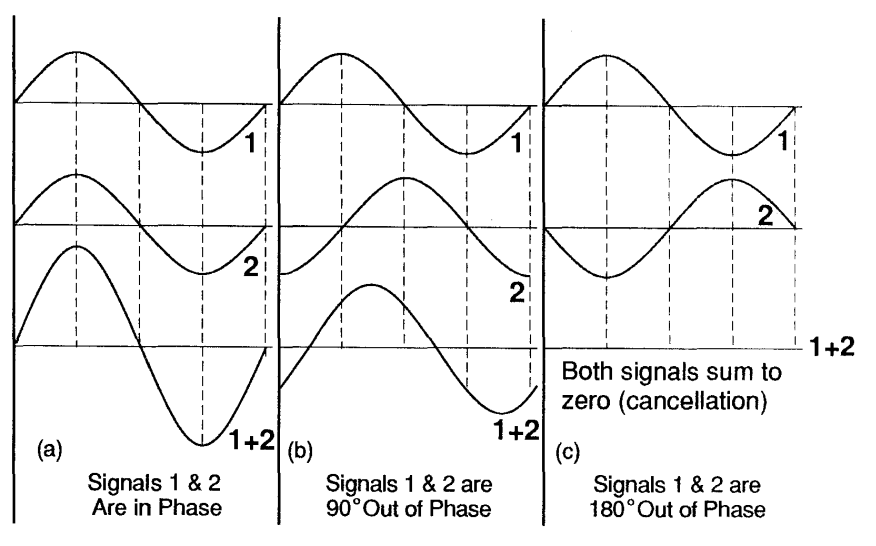
\includegraphics[width=0.75\textwidth]{phase.png}
\end{center}

When two sounds are added, we get interference. There are two types of
interference:
\begin{enumerate}
	\item Constructuve interference: the two waves are combining so that
		they're adding to each other---the resultant wave amplitude 
		in that location is greater than either of the waves
		individually
	\item Destructive interference: the two waves are combining so that
		they're subtracting from each other---the resultant wave
		amplitude in that location is smaller than one or both of the
		waves individually
\end{enumerate}
Maximum constructive/destructive interference happens when the waves double
each other or totally cancel each other out (respectively).

We can also apply this to pink noise: when we delay one pink noise signal
compared to another, it forces the resultant pink noise to have nodes (places
where certain frequencies are decreased). The farther apart we set the pink
noises, the more nodes we have and the lower they go, since lower frequencies
require a farther distance to be totally out of phase. This \emph{also} also
applies to sounds in general: voices, music, etc. At around 30-40ms later, we
hear it as a delay rather than a drequency response issue.

For loudspeakers, the ``problem path'' is where there's little difference in
volume, but noticeable time offsets, because this is what causes more intense
comb filtering. We prefer level offsets much more over time offsets, and level
offsets can help compensate for time offsets a little bit. This means we want
to minimize the region of overlap, because what's where we run into issues of
comb filtering (and echo, potentially).

With microphones, we talk about the 3:1 rule: however far your first
microphone is from a source, your second source should be at least 3x that
distance.

\subsection{Focus in Plan: Pan}

True stereo isn't really possible for more than a couple poeople at a time down
the center line of the speakers. It also gets less exciting the farther back
you go---very far back, the angular width of stereo differences gets pretty
small, and it's not really that exciting any more. For the people outside of
this range, a change in pan just winds up being a level change.

Bob McCarthy gives a rule, which we can use as a starting point but doesn't
always work, for how to place loudspeakers. He says to divide the audience in
two, then point the loudspeakers at the center of each of these halves.

Important: in the horizontal plane especially, parts of your system \emph{will}
overlap in coverage. The important thing to consider is the relationship
between level and arrival time: they should either be as similar as possible,
or as different as possible.

\subsection{Fill Systems in Plan: Extending Horizontal Coverage}

Like in the vertical plane, we figure out how to point the speakers for maximum
coverage (and minimum overlap), and add fill speakers where there is no
coverage to fill in the difference. Like with vertical fill systems, horizontal
fill systems are named pretty self-explanatorily, like center fill, side fill,
etc.

\part{Mix Engineering}

\section{Analog Mix Engineering}

\subsection{Bus Architecture}

A bus refers to console outputs. Buses are organizational tools that collect
audio inputs on route to a common destination. For example, if we want to send
a mix to the stage manager that's separate from the main mix, we could say that
those mixes are on two different buses. Buses are used in analog consoles,
digital consoles, recording studios, live sound, DAWs, etc. Although this is in
the analog console section, it's not specific to analog consoles, this is just
the first time it was convenient to bring it up.

There are a few basic types of busses, which we'll go over in more detail in
the following sections:
\begin{itemize}
	\item Aux (or variable send)
	\item Group (or fixed send)
	\item Stereo/mono (or master)
	\item Matrix
\end{itemize}

\subsubsection{Aux Bus}
Aux busses, also known as mix busses, are variable sends---this means that you
can control how much sound gets sent to this bus individually, as a function of
the fader and the aux send. Aux busses can only receive input channels. Aux
busses are usually used for effects sends (eg. reverb) or monitors.

\subsubsection{Group Bus}
Group busses are fixed sends---this means that you can't independently control
how much goes to the group bus, only whether or not sound is going to it. The
volume of the channel going to the group is just set by the fader. Group busses
can also only receive input channels. Group busses are typically used to group
channels together that are headed towards other output busses. A good example
is grouping up all the drum mics before sending them to the main output.

\subsubsection{Master Bus}
Also fixed sends, and also controlled by the main fader. Master busses can
receive any combination of input channels and output busses, unlike the last
two. When the term ``stereo bus'' is used to refer to these, it's ued in a
generic sense of the term (ie. two speakers), not the literal definition of
stereo.

\subsubsection{Matrix}
Matrices are variable send busses, but matrices can receive only some
combintion of output busses. The levels in the sends are a function of matrix
sends and the fader level. Matrices are basically aux busses, but for other
busses rather than input channels. These are typically used to combine output
busses to fill systems.

\subsubsection{Pre-Fade vs. Post-Fade}
This is only relavent for aux sends and matrix sends. These sends can be
pre-fade or post-fade. Pre-fade busses mean that the audio is diverted to the
aux bus before it's sent to the fader, so both the fader and the send get
the same input (ie. the send volume doesn't rely on the fader---the main mix
will have no effect on the bus). Post-fade
busses have audio diverted after the fader, so the input for the send is the
same as the output of the fader (ie. the send volume also relies on the
fader---changing the main mix will change the volume going to the bus as well).

\section[Additional Considerations]{Additional Considerations for the Engineer}

\subsection{RF Basics}
RF stands for radio frequency---it's the umbrella term for all wireless
devices. We're familiar with air traveling through air/water/etc as acoustical
signal (ie. pressure waves). We're also familiar with the idea of audio
travelling through cables as voltage information. RF is similar---the audio
signal moves through the air as electromagnetic signal (like light), which can
be decoded by the receiver. 

Like audio, the electromagnetic waves that the signal travels on has amplitude
and wavelength/frequency. Note that these refer to the characteristics of the
transmission, not the characteristics of the sounds they carry. Unlike sound
waves, RF waves travel
at the speed of light, and have some polarization (ie. the waves are aligned in
some axis)---this means that antennae have to be in the same direction of the
polarized signal.

RF transmission is referred to as TX, and receiving is referred to as RX.

Receivers work by taking a small band of frequencies in the EM spectrum and
listening to them. This is usually written as a single frequency, but in
reality, it's a narrow region around that frequency. Receivers have no way of
knowing whether what they're picking up is what it's supposed to be, or just
unrelated noise at that frequency. Our job is to make sure that the RF signal
is the strongest thing at that frequency so we don't have to worry about this.

Some types of attenas:
\begin{itemize}
	\item Whip antenna\\
		Most basic kinds, omnidirectional. Comes in half-wave and
		quarter-wave sizes. Quarter-waves are less precise, although
		tbh neither are particularly precise. They're fine if you don't
		have a lot of noise, but not very preferable otherwise.
	\item Log periodice (paddle, sharkfin)\\
		Cardioid directional pattern, roughly 150$^\circ$ wide.
	\item Helical\\
		Thinner conic pattern (60$^\circ$), picks up any polarization.
\end{itemize}

RF distro (distribution) allows one pair of antennas to feed multiple
receivers.

Bodies absorb RF really easily. We want to put our receivers high in the air,
giving it a good line of sight. In general, if an obstacle is small compared to
the wavelength of the signal, it won't affect it much, but if the obstacle is
large, it will block it much more. The inverse is true for windows or holes.

We
also sometimes need to worry about multi-path interference: that is, sometimes
RF signal
will reflect off of a surface, and antennas will pick up both the original
signal and the reflected signal. This is a lot like comb filtering: the two
signals are arriving out of phase, which can mean we have huge attenuation of
signal. This is why we can randomly lose signals in certain places. In order to
fix this, we worry about diversity: we keep multiple (usually 2) antennas at
one time, and the receiver will use the signal from whichever antenna is
getting the strongest signal. In order to achieve multi-path diversity, we
actually want to keep them pretty close to each other (they should be within
1/4 to 1 wavelength apart). In our RF operating ranges, this means 3-12 inches
for high frequencies and 12-46 inches for low frequencies. We can usually call
this ``about a rack width apart.''

There are other kinds of diversity we might want to pay attention to as well:
\begin{itemize}
	\item Coverage area\\
		You can have multiple antennas in two different areas, of one
		of the antennas can't cover the whole area. THere will still be
		multi-path dropout.
	\item  Polarization\\
		You can have one antenna vertically and one horizontally, so
		that if signal polarization changes, we can still get signal.
		We can combine this with multipath diversity by having both at
		45 degree angles.
	\item Obstacles\\
		Similar to coverage area, if there's going to be a big
		obstacle, we can use an antenna to compensate.
\end{itemize}

One last form of interference: intermods/intermodulation interference. Every
time we introduce a new transmitter, it introduces some ambient noise and
random peaks from interacting with the other frequencies, mucking up the RF
spectrum. The locations of these depends on the relationship between the
frequencies. The height depends on the distance between the transmitters. The
main solution is to calculate the intermods when selecting the operating
frequencies to make sure that we won't be getting intermods where we have other
devices operating. Fortunately, there's a lot of software that can calculate
this for you.

\subsection{Analog Patching}
Patching refers to plugging the output of one device into the input of another.
It refers to the signal flow between devices.
This is not to be confused with routing, which lays out the signal flow within
a single device. In a sound system, things don't need to be hard-patched to
each other in an inflexible way. We can include patchbays at various points in
the signal flow, allowing you to flexibly patch the flow where you want it.
This means that we can just plug inputs/outputs where it's most convenient and
patch them where they need to be, rather than needing to run it all the way to
the right channel when it might be more difficult that way.

Some patchbays operate in ``normal'' configuration. This means that there's a
default when no cables are plugged into the front, where the inputs and outputs
are correlated 1:1, and plugging in a patch cable overrides that internal
connection.

\section{Stages of Amplification}

\subsection{Gain Structure}
Throughout the audio signal chain, there are a lot of places to adjust gain
(ie. the strength of the electrical signal which correlates with volume). Where
and when do we want to be adding or removing gain? There are 4 big places to
change gain: preamp, volume fader, output fader, and amplifier. When you bring
up the signal too high at the early stage, it's easier to get clipping, and if
it's too low at an early stage, you wind up having to amplify later in the
signal chain, picking up all the extra noise in the system. Clipping can happen
at any point in the gain stage, but sometimes for different reasons (ie. if the
amp gain is too high and causes clipping, it's usually because the speakers
themselves are being driven too hard and might be damaged, but at the preamp
level, you're just trying to push through more voltage than it's able to). You
want to be up as loud as possible without clipping early in the signal chain
(leave yourself some headroom).

\subsection{Power Amplifiers}
Power amps (usually just called amps) come right before the speakers. Amps
convert line level signal (1-10 V) to speaker level signal (10-50 V). Amps are
not transiducers because they don't convert between types of energy, they just
modify the electrical signal.  Ideally, the amps don't do anything other than
make the sound signal louder (although they will always color the sound in some
way, like all components in the signal chain).

Stereo mode: each input goes to its respective output (1 to 1, 2 to 2). Bridged
mono: the first input goes to both outputs, the second input is ignored.
Bridged mono is useful because it can produce more power than stereo mode,
which is helpful for bigger speakers.

We can daisy-chain loudspeakers together: we can send the same signal to each
speaker in a chain by physically connecting them together. This assumes, of
course, that we have enough power coming from the speakers to do this for the
number of speakers we're trying to chain together. This will decrease the
impedance of the load by putting the speakers in parallel (ie. two 8 $\Omega$
speakers will have a total impedance of 4 $\Omega$). Usually, if we use more
than 3 loudspeakers on a single chain, we start getting into fire hazard
territory, so we don't want to go above that. The amp spec sheet will tell us
the power the amp can deliver to different impedances. If the amp doesn't give
a spec for a particular load, don't try it, because that can be a fire hazard
(ie. don't go lower than the minimum impedance listed).

We also have to consider how much power we're delivering to a loudspeaker,
usually called power handling, power rating, or power capacity
(but not always---just look for the measurement
in Watts). We want to make sure the amp isn't providing more power than the
speaker is able to handle, breaking the speaker. Many list stats for
continuous (rms), program, and peak power. Continuous refers to an indefinite
sine wave, program refers to a more complicated signal (a shorter speech/music
source, for example), and peak refers to an impulse response, like a snare drum
hit or a plosive in a speech.
When you're planning amps on a circuit,
always plan for the max (probably)---if the spec sheet tells you a max current
draw, that's also ideal.

In order to determine matching up speakers and amps, we need to first match up
the impedance of the loudpspeaker to the impedance ratings of the amps, and the
power capacity of the speaker vs the power driven by the amp to a speaker with
that impedance. As a rule of thumb, we want the peak power of the amp to be in
the ballpark of half of what the speaker can handle (anything more than that
runs potential damage to the speaker).

We also want to look at sensitivity, which tells us how loud a speaker is in
response to a given amount of power. It will be given as dB SPL 1W @ 1m
distance (ie. decibels of sound pressure level from a 1 Watt power delivery at
1 meter distance). Higher sensitivity speakers will be louder, lower
sensitivity will be quieter at a given power. We can easily calculate the level
at other distances using the inverse square law (-6 dB per doubling). We can
also calculate the level for other amounts of power by calculating the ratio of
power delivered against 1 W.

\section{Paperwork}
There are four pieces of paperwork we should be responsible for as systems
designers. The first two are our plan \& section plots like we've already
talked about, the other two are our patch list, and our block diagram/signal
flow diagram/system overview. These last two basically show the same
information, just in different forms (one in writing, one graphically).

The paperwork is an opportunity to share with your collaborators anything
they'll need to know---make sure to include everything they need to know (and
nothing they don't). The paperwork we're making here is largely used for
communication between the designer and the engineer, but, for example, the
plots will be used by other designers, technical directors, stage managers,
etc.

Audio paperwork is really poorly-standardized. There have been occassional
attempts to standardize it (most recently in 2008 by USITT for block diagrams,
the documentation for which is also in this folder),
but most have been pretty unsuccessful. Because of that, we should consider on
a case-by-case basis what we should include/exclude/label based on our audience
rather than just following some rote guidelines.

In our plots, we can (and usually should) include annotations--telling us, for
example, what kind of speaker we're looking at, how many there are if they're
stacked in that view, etc. In something like vectorworks, we use the Callout
tool on the sheet layer (NOT the design layer). In our annotation, include:
speaker number, speaker function, make/model, rigging.

The patchlist shows detailed written information showing the signal flow
between all the elements of the system (usually written in a spreadsheet). The
block diagram, similarly, is where we bring the patchbay visually to life.
Usually, each element is described with a labelled block, and every connected
item is connected with a line.

\section{Microphones}

\subsection{How Microphones Work}
Microphones are transducers: electronic components that comvert one type of
energy into another (in this case, from acoustical energy to electronic energy,
the opposite of speakers). There are three basic families of microphones:
\begin{enumerate}
	\item Condenser\\
		Condenser microphones consist of a small parallel-place
		capacitors (that is, two flat parallel conductors). The
		distance between the plates affects the voltage across the
		plates. Acoustical energy moves one of the plates, causing a
		change in voltage proportional to the vibrations of the
		acoustical energy. In order for this to work, though, we need
		some charge on the capacitors (which we do with phantom power,
		or sometimes just a battery). The diaphram of a condensor
		microphone can be very light, making them potentially much more
		sensitive (but also less durable).
	\item Dynamic\\
		Dynamic microphones, also called moving coil microphones,
		are the most basic kinds of microphones. The vibrations in air
		move a coil of wire around a magnet, which generates current
		proportional to the sound vibrations.
	\item Ribbon\\
		Ribbon microphones are the most complicated. In these, we have
		a magnet, and suspended in the middle of the magnet is a very
		thin strip of corrugated metal (the ribbon). Acoustic energy
		moves the ribbon in the magnetic field, generating a current,
		much like dynamic microphones.

\end{enumerate}

\subsection{Selection and Deployment of Microphones}

\subsection{Feedback}

\subsection{A:D and D:A Conversion}

\section{Digital Mix Engineering}

\subsection{DCA Assignments}

\subsection{Digital Consoles}

\section{Delaying Larger Systems}

\subsection{Input Delays}

\subsection{Delay Matrixing}

\subsection{Staging Zones}

\section[Concert Audio]{System Principles from Concert Audio}

\subsection{Subwoofer Deployment}

\subsection{Cardioid Subwoofers}

\subsection{Line Array Theory}

\section[Control Systems]{Control Systems and Networked Audio}

\subsection{MIDI, OSC}

\subsection{Networking Basics}

\subsection{Dante Overview}

\section[System Tuning]{System Tuning and Measurement Microphones}

\subsection{SMAART Software and Approach}

\end{document}
